% !TeX spellcheck = en_US
% !TeX document-id = {cf032f19-4427-4a50-b0ba-ddee651fb980}
% !TeX program = txs:///dvi-ps-pdf-chain
% TeX program = txs:///dvi-chain
%DVI -> PS -> PDF
% 10.1016/j.compstruc.2017.04.006 
% OJO VERIFICAR IDIOMA GB

%\documentclass[preprint,12pt,authoryear,letterpaper,times]{elsarticle}
%\documentclass[final,1p,times,twocolumn,authoryear]{elsarticle}
\documentclass[12pt,letterpaper, landscape]{article}

\usepackage{parskip} 
\usepackage[margin=3cm]{geometry}
\usepackage{parskip}
%\usepackage{times}
\usepackage{braket}
\usepackage{mathtools} \mathtoolsset{showonlyrefs} %show only referenced equations
%\usepackage[latin1]{inputenc}
\usepackage[utf8]{inputenc}
%\usepackage[T1]{fontenc}
\usepackage{psfrag}
\usepackage[spanish]{babel}
\usepackage{mathrsfs}  % mathscr
\usepackage{bbm} % R Q N Z symbols
\usepackage{url}
\usepackage{natbib}
\usepackage{amsmath,amssymb,amsthm,amsfonts}

% FOR USE WITH THE TODONOTES PACKAGE:
\usepackage{xcolor}
\usepackage[spanish,textwidth=2cm]{todonotes} %todonotes goes after xcolor (messages, what to do!)

\usepackage{graphicx}

\newcommand\todoin[2][]{\todo[inline, caption={2do}, #1]{\begin{minipage}{\textwidth-4pt}#2\end{minipage}}}

\newcommand{\pf}{P_\text{\textnormal{f}}}
\newcommand{\LP}{\underline{P_{\Gamma}}}
%\newcommand{\e}{{(e)}}
\newcommand{\e}{{}}
\newcommand{\ve}[1]{{\boldsymbol{#1}}}
\newcommand{\ma}[1]{{\boldsymbol{#1}}}
\newcommand{\dd}{\operatorname{d} \!}
%\newcommand{\nuevo}[1]{\textsf{\textcolor{red}{#1}}}
\newcommand{\nuevo}[1]{#1}
\def\bigtimes{\mathbin{\vcenter{\hbox{\Large $\times$}}}} %\mbox{\Large$\times$} = \bigtimes
%\newcommand{\nuevo}[1]{{#1}}

\newtheorem{thm}{Theorem}
\newtheorem{cor}{Corollary}

\usepackage[colorlinks=true,citecolor=blue,%
plainpages=false,pdfpagelabels,%
breaklinks]{hyperref}
\hypersetup{pdffitwindow=false}

\usepackage{hypernat} % in this way [sort&compress]{natbib} and hyperref will work together

\usepackage{breakurl}

\title{Deducción de la ecuación $\ma{K}^{(e)} \ve{a}^{(e)} - \ma{f}^{(e)} = \ma{q}^{(e)}$ para un EF bidimensional de $n$ nodos}
\date{}
\begin{document}
\maketitle

A continuación no se escribirá el superíndice ${}^{(e)}$, en varias de las ecuaciones, para evitar saturar la notación.

%\section{Se interpola la geometría utilizando las mismas funciones de forma que interpolan el desplazamiento}
%
%Se interpola la geometría utilizando las mismas funciones de forma que se emplearán para interpolar los desplazamientos:
%\begin{align}
%x^\e(x,y) 
%&= N_1^\e(x,y) x_1^\e + N_2^\e(x,y) x_2^\e + \cdots + N_n^\e(x,y) x_n^\e 
%= \sum_{i=1}^n N_i^\e(x,y) x_i^\e \\
%&= 
%\underbrace{\begin{bmatrix}
%    N_1^\e(x,y) & N_2^\e(x,y) & \cdots & N_n^\e(x,y)
%    \end{bmatrix}}_{\ma{N}^\e(x,y)}
%\underbrace{\begin{bmatrix}
%    x_1^\e \\ x_2^\e \\ \vdots \\ x_n^\e
%    \end{bmatrix}}_{\ma{x}^\e} = \ma{N}^\e(x,y)  \ve{x}^\e
%\end{align}
%
%\begin{itemize}
%    \item $\ma{N}^\e(x,y)$ se conoce como la \emph{matriz de funciones de forma (locales) del elemento} $e$.
%    \item $\ve{x}^\e$ es el \emph{vector de coordenadas nodales del elemento} $e$.
%\end{itemize}    
%
%
%
%Se calcula el jacobiano de la transformación
%\begin{align}
%J^\e(x,y) &= \frac{\dd x^\e(x,y)}{\dd \xi} = 
%\frac{\dd}{\dd \xi}\left(\sum_{i=1}^n N_i^\e(x,y) x_i^\e\right) = \sum_{i=1}^n \frac{\dd N_i^\e(x,y)}{\dd \xi} x_i^\e \\
%&= 
%\underbrace{\begin{bmatrix}
%    \frac{\dd N_1^\e(x,y)}{\dd \xi} & \frac{\dd N_2^\e(x,y)}{\dd \xi} & \cdots & \frac{\dd N_n^\e(x,y)}{\dd \xi}
%    \end{bmatrix}}_{\frac{\dd \ma{N}^\e(x,y)}{\dd \xi}}
%\underbrace{\begin{bmatrix}
%    x_1^\e \\ x_2^\e \\ \vdots \\ x_n^\e
%    \end{bmatrix}}_{\ma{x}^\e} \\
%&= \frac{\dd \ma{N}^\e(x,y)}{\dd \xi}  \ve{x}^\e
%\end{align}
%y utilizando el teorema de la función inversa (ver: \url{https://en.wikipedia.org/wiki/Inverse_function_theorem}), también la derivada:
%\begin{align}
%\frac{\dd \xi(x)}{\dd x} = \frac{1}{J^\e(\xi(x))}.
%\end{align}
%
%
%Recuerde que la transformación isoparamétrica es válida siempre y cuando $J^\e(x,y)>0$ en todos los puntos del EF. Esto garantiza que $x(x,y)$ sea una función biyectiva en el intervalo $\xi\in[-1,1]$.
%
%
%
%\newpage

\section{Se definen los campos vectoriales de desplazamientos y  de desplazamientos virtuales}
Se interpolan los desplazamientos al interior del EF:
\begin{alignat}{2}
u^\e(x,y) &= \sum_{i=1}^n N_i^\e(x,y) u_i^\e 
&&= N_1^\e(x,y) u_1^\e + N_2^\e(x,y) u_2^\e + \cdots + N_n^\e(x,y) u_n^\e  \\
v^\e(x,y) &= \sum_{i=1}^n N_i^\e(x,y) v_i^\e 
&&= N_1^\e(x,y) v_1^\e + N_2^\e(x,y) v_2^\e + \cdots + N_n(x,y) v_n.
\end{alignat}
Observe que se están empleando las mismas funciones de forma para interpolar los deplazamientos $u$ y $v$. De hecho, no existe razón alguna para utilizar funciones de forma diferentes para la interpolación de $u$ y de $v$. 

%\subsection{Funciones de forma para el EF triangular de 3 nodos}
%Dichas funciones de forma están dadas por:
%
%\begin{align}
%N_i^\e(x,y) = \frac{1}{2A^\e}\left(a_i + b_i x + c_i y\right) \quad \text{ para } i = 1,\ 2,\ 3
%\end{align}
%donde:
%\begin{align}
%***
%\end{align}
%y $A^\e$ representa el área del EF $(e)$, el cual está dada por:
%\begin{equation}
%xxx
%\end{equation}
%
%\subsection{Funciones de forma para el EF rectangular de 4 nodos}
%Dichas funciones de forma están dadas por:

Las ecuaciones anteriores se pueden escribir matricialmente como:
\begin{align}
\underbrace{\begin{bmatrix}
u^\e(x,y) \\
v^\e(x,y)
\end{bmatrix}}_{\ve{u}^\e(x,y)}
=
\underbrace{\begin{bmatrix}
N_1^\e(x,y) & 0 & N_2^\e(x,y) & 0   & \cdots & N_n^\e(x,y) & 0\\
0 & N_1^\e(x,y) & 0 & N_2^\e(x,y)   & \cdots & 0 & N_n^\e(x,y) 
\end{bmatrix}}_{\ma{N}^\e(x,y)}
\underbrace{\begin{bmatrix}
   u_1^\e \\ v_1^\e \\ u_2^\e \\ v_2^\e \\ \vdots \\ u_n^\e \\ v_n^\e
\end{bmatrix}}_{\ma{a}^\e},
\end{align}
es decir,
\begin{equation}
\ve{u}^{(e)}(x,y) = \ma{N}^{(e)}(x,y)  \ve{a}^{(e)}.
\end{equation}

%http://ctan.math.washington.edu/tex-archive/macros/latex/contrib/nicematrix/nicematrix.pdf

Análogamente, a como se hizo con el EF de barra, los desplazamientos virtuales al interior del elemento son:
\begin{align}
\delta u^\e(x,y) &= \sum_{i=1}^n N_i^\e(x,y) \delta u_i^\e &
\delta v^\e(x,y) &= \sum_{i=1}^n N_i^\e(x,y) \delta v_i^\e, 
\end{align}
y ambos se expresan en forma matricial como:
\begin{equation}
\delta \ve{u}^{(e)}(x,y) = \ma{N}^{(e)}(x,y)  \delta\ve{a}^{(e)}. \label{eq:delta_u}
\end{equation}

Los términos expresados en las ecuaciones anteriores son:

\begin{tabular}{ll}
$\ve{u}^{(e)}(x,y)$     & {campo vectorial de desplazamientos del elemento} $e$.\\
\\[-1ex]
$\ma{N}^{(e)}(x,y)$  & {matriz de funciones de forma (locales) del elemento} $e$.\\
\\[-1ex]
$\ve{a}^{(e)}$       & {vector de desplazamientos nodales del elemento} $e$. \\
\\[-1ex]
$\delta\ve{a}^{(e)}$ & {vector de desplazamientos virtuales nodales del elemento} $e$.
\end{tabular} 

\newpage

\section{Se definen los campos vectoriales de deformaciones y  de deformaciones virtuales}

Las deformaciones longitudinales del EF están dadas por:
\begin{alignat}{3}
\varepsilon^\e_x(x,y) &= \frac{\partial u^\e(x,y)}{\partial x} &&= \frac{\partial}{\partial x}\left(\sum_{i=1}^n N_i^\e(x,y) u_i^\e\right) &&= \sum_{i=1}^n \frac{\partial N_i^\e(x,y)}{\partial x} u_i^\e\\
\varepsilon^\e_y(x,y) &= \frac{\partial v^\e(x,y)}{\partial y} &&= \frac{\partial}{\partial y}\left(\sum_{i=1}^n N_i^\e(x,y) v_i^\e\right) &&=\sum_{i=1}^n \frac{\partial N_i^\e(x,y)}{\partial y} v_i^\e,
\end{alignat}
y las deformaciones angulares por:
\begin{equation}
\gamma^\e_{xy}(x,y) = \frac{\partial u^\e(x,y)}{\partial y} + \frac{\partial v^\e(x,y)}{\partial x} = \frac{\partial}{\partial x}\left(\sum_{i=1}^n N_i^\e(x,y) v_i^\e\right) + \frac{\partial}{\partial y}\left(\sum_{i=1}^n N_i^\e(x,y) u_i^\e\right) = \sum_{i=1}^n \frac{\partial N_i^\e(x,y)}{\partial x} v_i^\e + \sum_{i=1}^n \frac{\partial N_i^\e(x,y)}{\partial y} u_i,
\end{equation}
es decir,
\begin{alignat}{7}
\varepsilon_x &= +\frac{\partial N_1}{\partial x} u_1 &&                                     &&+ \frac{\partial N_2}{\partial x} u_2 &&                                      &&+\cdots &&+\frac{\partial N_n}{\partial x} u_n && \\
\varepsilon_y &=                                      &&+\frac{\partial N_1}{\partial y} v_1 &&                                      &&+ \frac{\partial N_2}{\partial y} v_2 &&+\cdots &&                                     && + \frac{\partial N_n}{\partial y} v_n \\
\gamma_{xy}   &= +\frac{\partial N_1}{\partial y} u_1 &&+\frac{\partial N_1}{\partial x} v_1 &&+ \frac{\partial N_2}{\partial y} u_2 &&+ \frac{\partial N_1}{\partial x} v_2 &&+\cdots &&+\frac{\partial N_n}{\partial y} u_n && + \frac{\partial N_n}{\partial x} v_n.
\end{alignat}
Las ecuaciones anteriores se pueden expresar en forma matricial como:
\begin{align}
\underbrace{\begin{bmatrix}
  \vphantom{\frac{\partial N_1^\e}{\partial x}} \varepsilon^\e_x \\
  \vphantom{\frac{\partial N_1^\e}{\partial y}} \varepsilon^\e_y \\
  \vphantom{\frac{\partial N_1^\e}{\partial y}} \gamma^\e_{xy}
\end{bmatrix}}_{\ve{\varepsilon}^\e(x,y)}=
\underbrace{\begin{bmatrix}
  \frac{\partial N_1^\e}{\partial x} & 0                                  & \frac{\partial N_2^\e}{\partial x} & 0 & \cdots & \frac{\partial N_n^\e}{\partial x} & 0 \\
   0                                 & \frac{\partial N_1^\e}{\partial y} & 0                                  & \frac{\partial N_2^\e}{\partial y} & \cdots & 0 & \frac{\partial N_n^\e}{\partial y}  \\
  \frac{\partial N_1^\e}{\partial x} & \frac{\partial N_1^\e}{\partial y} & \frac{\partial N_2^\e}{\partial x} & \frac{\partial N_2^\e}{\partial y} & \cdots &
\frac{\partial N_n^\e}{\partial x}   & \frac{\partial N_n^\e}{\partial y}
   \end{bmatrix}}_{\ma{B}^\e(x,y)} 
\underbrace{\begin{bmatrix}
   u_1^\e \\ v_1^\e \\ u_2^\e \\ v_2^\e \\ \vdots \\ u_n^\e \\ v_n^\e 
   \end{bmatrix},}_{\ma{a}^\e}
\end{align}
es decir,
\begin{align}
 \ve{\varepsilon}^{(e)}(x,y) = \ma{B}^{(e)}(x,y)  \ve{a}^{(e)}.
\end{align}

De forma análoga a como se hizo con el EF de barra, las deformaciones virtuales al interior del elemento están dadas por:

\begin{equation}
\delta \ve{\varepsilon}^{(e)}(x,y) = \ma{B}^{(e)}(x,y)  \delta  \ve{a}^{(e)}. \label{eq:delta_varepsilon}
\end{equation}

Los términos expresados en las ecuaciones anteriores son: 

\begin{tabular}{ll}
   $\ve{\varepsilon}^{(e)}(x,y)$     & campo vectorial de deformaciones del elemento $e$.\\
   \\[-1ex]
   $\ma{B}^{(e)}(x,y)$  & {matriz de deformaciones del elemento} $e$.\\
   \\[-1ex]
   $\ve{a}^{(e)}$       & {vector de desplazamientos nodales del elemento} $e$. \\
   \\[-1ex]
   $\delta\ve{a}^{(e)}$ & {vector de desplazamientos virtuales nodales del elemento} $e$.
\end{tabular} 

\newpage

\section{Se define el campo vectorial de esfuerzos}

Para un elemento finito sujeto a deformaciones y esfuerzos iniciales, el campo vectorial de esfuerzos está dado por:
\begin{align}
\ve{\sigma}^\e(x,y) &= \ma{D}^\e(x,y)\left(\ve{\varepsilon}^\e(x,y) - \ve{\varepsilon}_0^\e(x,y)\right) + \ve{\sigma}_0^\e(x,y) \\
&= \ma{D}(x,y)\left(\ma{B}^\e(x,y)\ve{a}^\e - \ve{\varepsilon}_0(x,y)\right)^\e + \ve{\sigma}_0(x,y)^\e,
\end{align}
es decir,
\begin{equation}
\ve{\sigma}^{(e)}(x,y) =  \ma{D}^{(e)}(x,y)^\e\ma{B}^{(e)}(x,y)\ve{a}^{(e)} - \ma{D}^{(e)}(x,y)\ve{\varepsilon}_0^{(e)}(x,y) + \ve{\sigma}_0^{(e)}(x,y). \label{eq:constitutiva}
\end{equation}

Tenga en cuenta que $\ve{\sigma}(x,y) = [\sigma_x(x,y),\ \sigma_y(x,y),\ \tau_{xy}(x,y)]^T$.

Aquí:

\begin{tabular}{ll}
   $\ve{\sigma}^{(e)}(x,y)$     & campo vectorial de esfuerzos del elemento $e$.\\
\\[-1ex]   
   $\ma{D}^{(e)}(x,y)$ & matriz constitutiva del elemento $e$. \\
\\[-1ex]
   $\ma{B}^{(e)}(x,y)$  & {matriz de deformaciones del elemento} $e$.\\
   \\[-1ex]
   $\ve{a}^{(e)}$       & {vector de desplazamientos nodales del elemento} $e$. \\
   \\[-1ex]
   $\ve{\varepsilon}_0^{(e)}(x,y)$ & campo vectorial de deformaciones iniciales del elemento $e$. \\
   \\[-1ex]
   $\ve{\sigma}_0^{(e)}(x,y)$ & campo vectorial de esfuerzos iniciales del elemento $e$.   
\end{tabular} 

\newpage

\section{Se reemplaza en el principio de los trabajos virtuales}

Haciendo $\ve{x} = [x,\ y]^T$, y teniendo en cuenta las fuerzas que se muestran en la Figura~\ref{eq:fuerzas_sobre_EF}, escribimos el PTV en 2D:
\begin{figure}[p]
   \centering   
   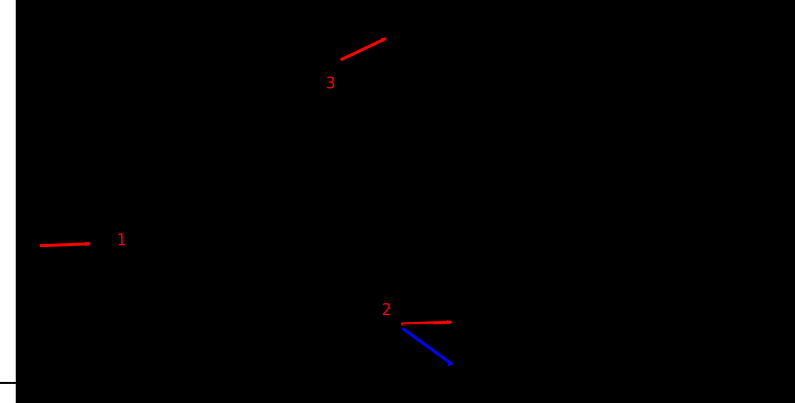
\includegraphics[width=\textwidth]{../codigo/2D/ejemplo_T3/figs/fuerzas_EF_T3}
   \caption{Fuerzas que actúan sobre un elemento finito}
   \label{eq:fuerzas_sobre_EF}
\end{figure}
\begin{equation}
\underbrace{t^\e \iint_{A^\e} \delta\ve{\varepsilon}_\e^T(\ve{x}) \ve{\sigma}^\e(\ve{x}) \dd A}_{\footnotesize\parbox{11em}{trabajo realizado por las deformaciones virtuales sobre los esfuerzos en el EF}}
 = \underbrace{t^\e \iint_{A^\e} \delta \ve{u}_\e^T(\ve{x}) \ve{b}^\e(\ve{x}) \dd A}_{\footnotesize\parbox{11em}{trabajo realizado por las fuerzas másicas sobre los desplazamientos virtuales en el EF}}
+ \underbrace{t^\e \oint_{\partial A^\e} \delta \ve{u}_\e^T(\ve{x}(s)) \ve{t}^\e(\ve{x}(s)) \dd s}_{\footnotesize\parbox{13em}{trabajo realizado por las fuerzas superficiales (que actúan en el contorno del EF) sobre los desplazamientos virtuales en el EF}}
+ \underbrace{\sum_{i=1}^n \delta \ve{u}_\e^T(\ve{x}_i) \ve{p}_i^\e}_{\footnotesize\parbox{9em}{trabajo realizado por las fuerzas puntuales aplicadas sobre los nodos del EF sobre sus correspondientes desplazamientos virtuales}}
+ \underbrace{\sum_{i=1}^n \delta \ve{u}_\e^T(\ve{x}_i) \ve{q}_i^\e.}_{\footnotesize\parbox{7em}{trabajo realizado por las fuerzas nodales de equilibrio sobre los desplazamientos virtuales de los nodos del EF}} \label{eq:PTV}
\end{equation}
donde: 

\begin{tabular}{ll}
   $t^{(e)}$     & espesor del elemento $e$.\\
   \\[-1ex]   
   $A^{(e)}$     & región del plano asociada al EF $e$, sobre la cual se realiza la integración.\\
   \\[-1ex]
   $\ve{\sigma}^{(e)}(x,y)$     & campo vectorial de esfuerzos del elemento $e$.\\
   \\[-1ex]   
   $\ve{b}^{(e)}(x,y)$ & vector de fuerzas másicas asociadas al elemento $e$.\\
   \\[-1ex]
   $\ve{t}^{(e)}(x(s),y(s))$  & vector de fuerzas superficiales que actúan en el contorno del elemento $e$.\\
   \\[-1ex]
   $\ve{p}_i^{(e)}$       & vector de fuerzas puntuales aplicadas sobre el nodo $i$-ésimo del EF $e$.\\
   \\[-1ex]
   $\ve{q}_i^{(e)}$ & vector de fuerzas nodales de equilibrio del nodo $i$-ésimo del EF $e$.\\
   \\[-1ex]
   $\delta\ve{u}_i^{(e)}$ & vector de desplazamiento virtual asociado al nodo $i$-ésimo del elemento $e$.\\
   \\[-1ex]      
   $\delta\ve{\varepsilon}^{(e)}(x,y)$     & campo vectorial de deformaciones virtuales del elemento $e$.
\end{tabular} 


Observe que $\delta\ve{\varepsilon}\ve{\sigma} := \sigma_x\delta\varepsilon_x + 
\sigma_y\delta\varepsilon_y +
\tau_{xy}\delta\gamma_{xy} +
\overbrace{\sigma_z\delta\varepsilon_z +
\tau_{xz}\delta\gamma_{xz} +
\tau_{yz}\delta\gamma_{yz}}^{=0}.$ El término señalado vale cero ya que en tensión plana $\sigma_z=\tau_{xz}=\tau_{yz}=0$ y en deformación plana $\varepsilon_z=\gamma_{xz}=\gamma_{yz}=0$.

A partir de las ecuaciones \eqref{eq:delta_u} y \eqref{eq:delta_varepsilon}, y teniendo en cuenta que $(\ma{A}\ma{B})^T = \ma{B}^T\ma{A}^T$,  se obtiene:
\begin{align}
 \delta \ve{u}^T(\ve{x}) &= \delta\ve{a}^T \ma{N}^T(\ve{x}) &
 \delta \ve{\varepsilon}^T(\ve{x}) = \delta\ve{a}^T \ma{B}^T(\ve{x}).
\end{align}
Reemplazando las dos ecuaciones anteriores en~\eqref{eq:PTV}, resulta:
\begin{equation}
t^\e \iint_{A^\e} \delta\ve{a}^T \ma{B}^T(\ve{x})  \ve{\sigma}^\e(\ve{x}) \dd A = t^\e \iint_{A^\e} \delta\ve{a}^T \ma{N}^T(\ve{x}) \ve{b}^\e(\ve{x}) \dd A 
+  t^\e \oint_{\partial A^\e} \delta\ve{a}^T \ma{N}^T(\ve{x}(s)) \ve{t}^\e(\ve{x}(s)) \dd s  
+ \sum_{i=1}^n \delta \ve{u}_\e^T(\ve{x}_i) \ve{p}_i^\e + \sum_{i=1}^n \delta \ve{u}_\e^T(\ve{x}_i) \ve{q}_i^\e. \label{eq:PTV2}
\end{equation}

Ahora, teniendo en cuenta que:
\begin{align}
\ve{p} &= \begin{pmatrix}
\ve{p}_1 \\ \ve{p}_2 \\ \vdots \\ \ve{p}_n
\end{pmatrix}
&
\ve{q} &= \begin{pmatrix}
\ve{q}_1 \\ \ve{q}_2 \\ \vdots \\ \ve{q}_n
\end{pmatrix}
&
\ve{a} &= \begin{pmatrix}
\ve{a}_1 \\ \ve{a}_2 \\ \vdots \\ \ve{a}_n
\end{pmatrix} = 
\begin{pmatrix}
\ve{u}(\ve{x}_1) \\ \ve{u}(\ve{x}_2) \\ \vdots \\ \ve{u}(\ve{x}_n)
\end{pmatrix}
&
\delta\ve{a} &= \begin{pmatrix}
\delta\ve{a}_1 \\ \delta\ve{a}_2 \\ \vdots \\ \delta\ve{a}_n
\end{pmatrix}
 = 
\begin{pmatrix}
\delta\ve{u}(\ve{x}_1) \\ \delta\ve{u}(\ve{x}_2) \\ \vdots \\ \delta\ve{u}(\ve{x}_n)
\end{pmatrix}
\end{align}
resulta que
\begin{align}
\sum_{i=1}^n \delta \ve{u}_\e^T(\ve{x}_i) \ve{p}_i^\e &= \delta\ve{a}^T \ve{p} &\sum_{i=1}^n \delta \ve{u}_\e^T(\ve{x}_i) \ve{q}_i^\e &= \delta\ve{a}^T \ve{q}.
\end{align}

Al reemplazar dichos términos en~\eqref{eq:PTV2} y pasando la parte derecha de la ecuación a la parte izquierda, obtenemos:
\begin{align}
t^\e \iint_{A^\e} \delta\ve{a}^T \ma{B}^T(\ve{x}) \ve{\sigma}^\e(\ve{x}) \dd A - t^\e \iint_{A^\e} \delta\ve{a}^T \ma{N}^T(\ve{x}) \ve{b}^\e(\ve{x}) \dd A 
-  t^\e \oint_{\partial A^\e} \delta\ve{a}^T \ma{N}^T(\ve{x}(x)) \ve{t}^\e(\ve{x}(s)) \dd s  
- \delta\ve{a}^T \ve{p} - \delta\ve{a}^T \ve{q} = 0. \label{eq:PTV3}
\end{align}

En la ecuación anterior, el desplazamiento virtual es independiente de los integrandos de todas las integrales, por lo que sale de la integral y se factoriza para quedar:
\begin{equation}
\underbrace{\vphantom{\Bigg[}\delta\ve{a}^T}_{\neq\ve{0}} \underbrace{\Bigg[ t^\e \iint_{A^\e} \ma{B}^T(\ve{x}) \ve{\sigma}^\e(\ve{x}) \dd A - t^\e \iint_{A^\e}  \ma{N}^T(\ve{x}) \ve{b}^\e(\ve{x}) \dd A - t^\e \oint_{\partial A^\e} \ma{N}^T(\ve{x}(x)) \ve{t}^\e(\ve{x}(s)) \dd s - \ve{p} - \ve{q} \Bigg]}_{=\ve{0}}= 0. \label{eq:PTV3}
\end{equation}

Si el producto punto anterior vale cero es porque $\delta\ve{a} = \ve{0}$ o porque el término entre corchetes es igual a $\ve{0}$. Lo primero no es cierto, ya que se sabe que el desplazamiento virtual $\delta \ve{a}$ representa el conjunto de todos los desplazamientos posibles de los nodos del EF, es decir, es un vector arbitrario. En consecuencia el término entre corchetes es cero y:
\begin{equation}
 t^\e \iint_{A^\e}  \ma{B}^T(\ve{x})  \ve{\sigma}^\e(\ve{x}) \dd A - t^\e \iint_{A^\e}  \ma{N}^T(\ve{x}) \ve{b}^\e(\ve{x}) \dd A -  t^\e \oint_{\partial A^\e} \ma{N}^T(\ve{x}(s)) \ve{f}^\e(\ve{x}(s)) \dd s -  \ve{p} - \ve{q} = \ve{0}.
\end{equation}

Al reemplazar~\eqref{eq:constitutiva} en la ecuación anterior, se obtiene
\begin{equation}
t^\e \iint_{A^\e}  \ma{B}^T(\ve{x}) \big(\ma{D}(\ve{x})\ma{B}(\ve{x})\ve{a}^\e - \ma{D}(\ve{x})\ve{\varepsilon}_0(\ve{x}) + \ve{\sigma}_0(\ve{x})\big) \dd A 
- t^\e \iint_{A^\e}  \ma{N}^T(\ve{x}) \ve{b}^\e(\ve{x}) \dd A -  t^\e \oint_{\partial A^\e} \ma{N}^T(\ve{x}(s)) \ve{f}^\e(\ve{x}(s)) \dd s -  \ve{p} - \ve{q} = \ve{0},
\end{equation}
es decir,
\begin{multline}
\underbrace{t^\e \iint_{A^\e}  \ma{B}^T(\ve{x})\ma{D}(\ve{x})\ma{B}(\ve{x}) \dd A}_{\ma{K}} \ve{a}^\e
% 
- \underbrace{t^\e \iint_{A^\e}  \ma{B}^T(\ve{x})\ma{D}(\ve{x})\ve{\varepsilon}_0(\ve{x}) \dd A}_{\ve{f}_{\ve{\varepsilon}_0}} 
%
- \underbrace{\left(-t^\e \iint_{A^\e}  \ma{B}^T(\ve{x})\ve{\sigma}_0(\ve{x}) \dd A \right)}_{\ve{f}_{\ve{\sigma}_0}} \\
%
- \underbrace{t^\e \iint_{A^\e}  \ma{N}^T(\ve{x}) \ve{b}^\e(\ve{x}) \dd A}_{\ve{f}_\ve{b}}
%
- \underbrace{t^\e \oint_{\partial A^\e} \ma{N}^T(\ve{x}(s)) \ve{f}^\e(\ve{x}(s)) \dd s}_{\ve{f}_\ve{t}} 
%
- \ve{p} = \ve{q},
\end{multline}
lo cual se expresa de forma compacta como:
\begin{equation}
\ma{K}^{(e)} \ve{a}^{(e)} - \ma{f}^{(e)} = \ma{q}^{(e)},
\end{equation}
donde,

\begin{tabular}{lp{14.2cm}}
   $\displaystyle \ma{K}^{(e)} = t^\e \iint_{A^\e}  \ma{B}^T(\ve{x})\ma{D}(\ve{x})\ma{B}(\ve{x}) \dd A$ & matriz de rigidez del elemento $e$.\\
   \\[-1ex]
   $\ve{a}^{(e)}$ & vector de desplazamientos nodales del elemento $e$.\\
   \\[-1ex]
   $\ma{f}^{(e)} = \ve{f}_{\ve{\varepsilon}_0}^{(e)} + \ve{f}_{\ve{\sigma}_0}^{(e)} + \ve{f}^{(e)}_\ve{b} + \ve{f}^{(e)}_\ve{t} + \ve{p}^{(e)}$     &  vector de fuerzas nodales equivalentes del elemento $e$.\\
   \\[-1ex]
   $\ve{q}^{(e)}$ & vector de fuerzas nodales de equilibrio del EF $e$.\\   
   \\[-1ex]
   $\displaystyle\ve{f}^{(e)}_{\ve{\varepsilon}_0} = t^\e \iint_{A^\e}  \ma{B}^T(\ve{x})\ma{D}(\ve{x})\ve{\varepsilon}_0(\ve{x}) \dd A$      & vector de fuerzas nodales equivalentes del elemento $e$ asociado a las deformaciones iniciales.\\
   \\[-1ex]   
   $\displaystyle \ve{f}^{(e)}_{\ve{\sigma}_0} = -t^\e \iint_{A^\e}  \ma{B}^T(\ve{x})\ve{\sigma}_0(\ve{x}) \dd A$ &vector de fuerzas nodales equivalentes del elemento $e$ asociado a los esfuerzos iniciales.\\
   \\[-1ex]
   $\displaystyle \ve{f}^{(e)}_\ve{b} = t^\e \iint_{A^\e}  \ma{N}^T(\ve{x}) \ve{b}^\e(\ve{x}) \dd A$ &vector de fuerzas nodales equivalentes del elemento $e$ asociado a las fuerzas másicas.\\
   \\[-1ex]
   $\displaystyle \ve{f}^{(e)}_\ve{t} = t^\e \oint_{\partial A^\e} \ma{N}^T(\ve{x}(s)) \ve{f}^\e(\ve{x}(s)) \dd s$ &vector de fuerzas nodales equivalentes del elemento $e$ asociado a las fuerzas superficiales actuantes en el contorno del EF.\\
\\[-1ex]   
   $\ve{p}^{(e)}$       & vector de fuerzas puntuales aplicadas sobre los nodos del EF $e$.
\end{tabular} 

\vspace{\baselineskip}\vspace{\baselineskip}
Hay que destacar que estas expresiones son totalmente generales y, por consiguiente, aplicables a cualquier elemento bidimensional.

Finalmente, tenga en cuenta que las ecuaciones anteriores solo involucran hasta las derivadas primeras del desplazamiento; por lo tanto, es posible utilizar elementos finitos continuos de clase $C_0$. Este requisito aplicará también para el caso tridimensional, pero no para el caso de vigas, placas y cascarones.

NOTA: la matriz $\ma{K}^{(e)}$ es simétrica y semi-positiva definida. Tiene tres valores propios nulo asociados con las dos translaciones rígidas y con la rotación. El rango de $\ma{K}^{(e)}$ es $2n-3$; este rango puede disminuir si se integra la matriz numéricamente con integración reducida.


%En las páginas anteriores se calculó $\ma{N}^\e$, $\ma{B}^\e$ y $\ma{D}^\e$ en función de $\xi$, por lo que es necesario hacer un cambio de variables en las integrales anteriores. De este modo:
%\begin{align}
%\ma{K}^\e &= \int_{-1}^{+1} \ma{B}_\e^T(x,y) \ma{D}^\e(x,y) \ma{B}^\e(x,y) \frac{\dd x^\e(x,y)}{\dd \xi} \dd \xi\\
%\ma{f}^\e &= \int_{-1}^{+1}  \ma{N}_\e^T(x,y) b^\e(x,y) \frac{\dd x^\e(x,y)}{\dd \xi} \dd \xi
%\end{align}
%
%Finalmente, se aproximan dichas integrales utilizando una cuadratura de $M$ puntos de Gauss-Legendre:
%\begin{align}
%\ma{K}^\e &\approx \sum_{m=1}^M \ma{B}_\e^T(\xi_m) \ma{D}^\e(\xi_m) \ma{B}^\e(\xi_m) \frac{\dd x^\e(\xi_m)}{\dd \xi} w_m\\
%\ma{f}^\e &\approx \sum_{m=1}^M  \ma{N}_\e^T(\xi_m) b^\e(\xi_m) \frac{\dd x^\e(\xi_m)}{\dd \xi} w_m
%\end{align}
%
%Se deja como ejercicio al lector demostrar que:
%\begin{align}
%\ma{K}^\e_{pq} &\approx \sum_{m=1}^M \frac{\dd N_p(\xi_m)}{\dd \xi} E^\e(\xi_m) A^\e(\xi_m) \frac{\dd N_q(\xi_m)}{\dd \xi} \frac{1}{J^\e(\xi_m)} w_m\\
%\ma{f}^\e_p &\approx \sum_{m=1}^M  N_p^\e(\xi_m) b^\e(\xi_m) J^\e(\xi_m) w_m
%\end{align}
%donde $p, q = 1,\ 2, \ \ldots,\ n$.
\end{document}
